\begin{abstract}
Rerankers decide which passages a retrieval-augmented generation (RAG) system shows to its generator, and adapting them requires relevance labels. Document-level labels come free with question--answer data but are coarse: they mark every passage of the correct document as relevant, even when it lacks the answer. Labels that instead reward passages containing the reference answer verbatim look more precise. We put this literal-match supervision to a controlled test, with a fixed generator and a success criterion set in advance: a statistically significant gain of at least one point in answer F1 (word overlap with the reference answer). In neither study does it deliver that gain. On 208 held-out TechQA technical-support questions, it improves passage ranking over hybrid retrieval, but the answer gain is not significant ($\SoneDelta$ points). Under transfer to support dialogues (Doc2Dial), it ranks evidence worse than document-level labels and gives slightly lower answer F1 ($\StwoDelta$ points); for the trained adapters, the targeted gain is ruled out. A second finding holds across both studies: clear differences in retrieval quality barely move answer F1, which also tracks response length. Retrieval metrics are therefore an unreliable guide here, and reranker supervision should be judged by the answers it produces, using an answer metric shown to detect retrieval changes.
\end{abstract}
\noindent\textbf{Keywords:} retrieval-augmented generation; reranking; weak supervision; technical support; external transfer; negative results.

\section{Introduction}
In retrieval-augmented generation (RAG), a language model answers a question from passages selected by a retrieval pipeline \citep{lewis2020}. In technical-support systems the passages come from product documentation, and the reranker makes the final selection: it reorders a pool of retrieved candidates and decides which few passages the generator sees. Adapting the reranker to the target documentation is therefore a natural way to improve answers. Adaptation needs relevance labels, and existing question--answer data can supply two kinds without new~annotation.

The first kind, \emph{document-level labels}, marks every passage of the annotated gold document as relevant. These labels are coarse, because retrieving the right document does not guarantee that the selected passage contains the details a user needs. In the constructed example of Table~\ref{tab:toy}, a passage that lists supported versions counts as just as relevant as the passage that tells the user to restart the monitoring agent. The second kind, \emph{literal-match labels}, favors passages that contain the reference answer verbatim, a distant-supervision heuristic that has also been used to train dense retrievers \citep{karpukhin2020}. Literal-match labels therefore look like the more targeted signal. Unlike approaches that obtain the supervision signal for retrieval from a language model, through its feedback \citep{shi2024}, through joint training of ranking and generation \citep{yu2024} or through LLM utility annotations \citep{zhang2025utility}, they involve no language model. This paper tests whether that signal produces better answers.

Three considerations qualify that appeal. First, literal containment is only a lexical proxy for evidential support: it misses paraphrased or scattered evidence and can mishandle numbers, commands and version strings. Second, literal-match labels change the training data, not only the label values. Training is contrastive: each positive passage is scored against a small group of negatives. Under literal-match labels, when a question has a passage that contains the literal answer, gold-document passages that lack it become negatives. In Table~\ref{tab:toy}, for example, passages $c_2$ and $c_3$ are positives under document-level labels but negatives under literal-match labels, a reversal we call negative inversion (Section~\ref{sec:labels}). The labeling rule also changes how many training groups each question contributes. As a result, a reranker trained with literal-match labels differs in three respects from one trained with document-level labels: which passages it learns to demote, which questions contribute training groups and how often each group is seen. Its effects therefore cannot be attributed to label granularity alone. What we evaluate is the \emph{literal-match supervision pipeline}: the labels together with the training groups and training exposure they induce.

Third, a more targeted label need not produce better answers. \citet{salemi2024} found that query--document relevance labels correlate only weakly with downstream RAG performance, which suggests that a change in reranker supervision should be judged by the answers it produces, not by retrieval metrics alone.

We therefore evaluate literal-match supervision end to end. A candidate passage receives grade~2 if it contains the normalized reference answer, grade~1 if it comes from a gold document but does not contain the answer, and grade~0 otherwise. We compare a reranker adapted with these literal-match labels (L) with one adapted with binary document-level labels (B), and with two baselines that involve no adaptation: hybrid retrieval without reranking (H) and the unadapted reranker (U). The retrieval pipeline and the generator are held fixed. We address three research questions:
\begin{enumerate}[label=\textbf{RQ\arabic*},leftmargin=3em]
\item Does a reranker adapted with literal-match labels improve generated answers over hybrid retrieval on held-out in-domain questions?
\item Under transfer to a different support domain, does literal-match supervision yield better generated answers than document-level supervision?
\item How strongly do differences in retrieval quality propagate to differences in answer F1?
\end{enumerate}

We answer them in two studies, each with a protocol frozen before its own comparative outcomes existed. \textbf{Study~1 (in-domain)} adapts the literal-match reranker on TechQA \citep{castelli2020} and compares it with H on a reserve set of 208 TechQA questions held out from model selection. This reserve set had been partly exposed in earlier project work, and we could not establish a demonstrably unexposed TechQA evaluation set. \textbf{Study~2 (transfer)} therefore trains on the same TechQA development data and evaluates on 273 documents from the Doc2Dial support-dialogue dataset \citep{feng2020}, one dialogue turn per document, comparing all four methods; B and L are each trained with three seeds and the same number of training updates. Because the two studies differ in comparators, evaluation populations and limitations, we report them separately and neither pool them nor treat them as replications.

Both studies score the generator's answers with token F1 against a reference and use the same prespecified success criterion: an observed gain of at least $+1$ F1 point with two-sided $p<0.05$. Neither study met it, but the two outcomes differ. In Study~1 (RQ1), L improved NDCG@4 over hybrid retrieval, yet its answer-level gain was small and not statistically significant; the data neither confirm nor exclude the targeted gain. In Study~2 (RQ2), L had lower NDCG@4 on annotated evidence than B for every training seed and slightly lower answer F1; conditional on the trained adapters (that is, without accounting for variation from retraining with new seeds), the 95\% interval for the answer difference excludes the targeted gain. Across both studies (RQ3), clear differences in NDCG@4 came with small or nonsignificant differences in answer F1, and in Study~2 the answer differences tracked response length more closely than retrieval quality. We cannot fully tell whether retrieval differences propagate only weakly to the answers or whether token F1 is too insensitive to register the changes that do occur (Section~\ref{sec:evaluation}).

These answer-level results are specific to the literal-match supervision pipeline as tested, but the weak link between retrieval and answer differences also carries a lesson for evaluation: the results suggest that, in this setting, retrieval metrics alone were not a sufficient guide to answer-level outcomes.

Our contributions are as follows:
\begin{itemize}[leftmargin=*]
\item An end-to-end comparison of two reranker supervision pipelines judged by generated answers, with frozen protocols, transfer to a different support domain and, in the transfer study, three paired training seeds.
\item Answer-level results for the literal-match supervision pipeline under these protocols: no demonstrated improvement in either study, with an unresolved in-domain effect (RQ1) and, under transfer, an interval that excludes the targeted gain conditional on the trained adapters (RQ2).
\item Evidence from both studies on how retrieval quality, answer F1 and response length relate, and on what this implies for evaluating reranker supervision (RQ3).
\item A record of the design features that limit interpretation, including the partial prior exposure of the Study~1 reserve set, coupled differences in training exposure and an interval that is conditional on the trained adapters (Section~\ref{sec:limitations}). Post hoc analyses are labeled as such, and code and aggregate results are released.
\end{itemize}

\section{Related work}
\paragraph{Where the supervision signal comes from.} The original RAG framework combines a neural retriever with a generator for knowledge-intensive tasks \citep{lewis2020}, and several later methods take the training signal for retrieval from a language model. REPLUG keeps a black-box language model frozen and trains a dense retriever toward the documents that most improve that model's likelihood of the reference output \citep{shi2024}. RankRAG instruction-tunes a single language model both to rank contexts and to generate answers, so the ranker and the generator are the same model \citep{yu2024}. The utility-focused annotation study of \citet{zhang2025utility} has an LLM judge which passages are useful and trains retrievers on those judgments. In each case the language model takes part in supervising retrieval, through its feedback, through joint training or through its annotations. In our setting it does not: a separate reranker is adapted with fixed, deterministic labels while the generator stays unchanged, so that only the reranker's training differs between methods.

\paragraph{Answer containment as a relevance label.} Treating passages that contain the answer as relevant, the idea behind literal-match labels, is a classic way to obtain retrieval supervision without passage annotation. Dense Passage Retrieval uses such passages as positives when gold passages are not annotated \citep{karpukhin2020}, FILCO selects useful context for RAG with string inclusion, lexical overlap and conditional cross-mutual information before training a context filter \citep{wang2023filco}, and part of RankRAG's ranking data treats retrieved contexts that contain the answer as relevant \citep{yu2024}. In each of these uses, containment stands in for passage annotation within a larger training procedure. The comparison made here is narrower: containment-based labels against document-level labels for adapting a reranker that feeds a fixed generator, judged by the generated answer.

\paragraph{Training with several positives.} Containment and document-level labels can both give one question several positives, and how a loss treats them matters: \citet{zhang2025utility} report that the way multiple positives enter the loss affects retrieval quality. They train on MS MARCO-derived data with LLM-generated utility annotations and a loss that accommodates multiple positives through summed marginal likelihood. Our training instead builds a separate group for each highest-grade passage, so each positive is scored only against lower-grade negatives rather than sharing probability mass with the other positives (Section~\ref{sec:labels}). Our conclusions therefore concern this literal-match pipeline and the training groups it induces, not LLM utility annotation or semantic support labels in general. The reranker itself is built from existing components, the Qwen3 reranker family \citep{zhang2025qwen} and low-rank adaptation (LoRA) \citep{hu2021}, and we make no state-of-the-art claim.

\paragraph{Retrieval quality and answer quality.} Several studies bear on whether retrieval quality, as measured by relevance labels, predicts answer quality. eRAG responds to the weak correlation between query--document relevance labels and downstream RAG performance by labeling each retrieved document with the quality of the answer generated from it \citep{salemi2024}. \citet{cuconasu2024} show that the composition of the retrieved context can itself affect generation quality, and \citet{wang2024} compare existing retrieval, reranking and other pipeline modules by their effect on end-to-end RAG performance. RAGAs and ARES assess retrieval and context properties separately from answer quality using automated judges \citep{es2024,saad2024}. We also keep retrieval quality and answer quality apart, but without model judges: literal containment, NDCG@4 and answer token F1 are reported as separate measurements, and RQ3 asks how differences in retrieval relate to differences in answers.

\paragraph{Testing with dependent evaluation units.} \citet{dror2018} note that NLP test sets often violate independence because examples can come from the same source or document. Our paired bootstrap intervals and sign-flip tests treat the resampled units as independent, and the sign-flip tests also assume that, under the null hypothesis, each unit's paired difference is symmetric around zero. We therefore average the repeated chunker and seed records within each question or document before testing, and in Study~2 we resample and flip signs for whole families of related documents (Section~\ref{sec:study2}).

\section{Methods}\label{sec:pipeline}
Figure~\ref{fig:design} summarizes the design.

\subsection{Retrieval and generation pipeline}
Every method is run with four fixed chunkers: fixed-length 128 tokens with 19-token overlap, fixed-length 254 tokens with 38-token overlap, recursive 254 tokens with 38-token overlap, and sentence-based 254 tokens without overlap, with token limits from the all-MiniLM-L6-v2 tokenizer. For each query and chunker, sparse BM25 and dense retrieval each return 20 passages; dense retrieval uses BAAI/bge-small-en-v1.5 with its query prefix. Weighted reciprocal-rank fusion (weights 0.4 sparse and 0.6 dense; fusion constant 60) ranks the union of the two lists and keeps a common pool of 20 candidates per query and chunker. Fusion ties and other implementation details are given in \supp{S2}{supp:impl}. In Study~1 the query is the question; in Study~2 it is the dialogue history.

At inference time, the four methods differ only in how they order this common pool. H returns the fused ranking. U reranks the pool with the unadapted Qwen3-Reranker-0.6B, and B and L rerank it with LoRA adapters on the same model. The reranker instruction asks for passages with sufficient answer evidence, but the training labels are not judgments of semantic sufficiency. Each method passes its top four passages to a fixed Qwen3.5-9B generator (greedy decoding, thinking disabled, bfloat16, at most 1,536 input and 512 new tokens, batch size four; model revisions and prompts in \supp{S2}{supp:impl}).

Long inputs are truncated differently at each stage. The dense retriever and the reranker keep the first 512 tokens, so a long dialogue history can lose its most recent turns and an overlength passage loses its end. Training, by contrast, discarded query--passage pairs longer than 512 tokens. The number of truncated retrieval and reranker inputs at inference was not recorded (\supp{S2}{supp:impl}). The generator keeps the full question or history and shortens the context~instead.
\begin{figure}[htbp]\centering
\begin{tikzpicture}[
  box/.style={draw=black!60, rounded corners=2pt, align=center, font=\small, inner sep=5pt,
              execute at begin node={\hyphenpenalty=10000}},
  study/.style={box, fill=black!4},
  arr/.style={-{Stealth[length=2.2mm]}, black!70, thick}]
\node[box, text width=3.5cm] (data) {\textbf{TechQA development}\\400 questions\\(200 train, 200 validation)};
\node[box, text width=8.2cm, right=0.8cm of data] (adapt) {\textbf{LoRA adaptation of Qwen3-Reranker-0.6B}\\
  B: document-level labels; L: literal-match labels\\
  Study~1: L, three seeds (answers for one)\\Study~2: B and L, three seeds each};
\node[study, text width=5.6cm, below=0.9cm of data.south west, anchor=north west] (s1)
  {\textbf{Study 1 (in-domain)}\\TechQA reserve, 208 questions\\Compare L with H};
\node[study, text width=5.6cm, right=0.8cm of s1] (s2)
  {\textbf{Study 2 (transfer)}\\Doc2Dial, 273 dialogue turns\\Compare H, U, B and L (primary: L vs B)};
\node[box, text width=12.6cm, below=0.8cm of s1.south west, anchor=north west] (pipe)
  {Each method: hybrid retrieval (BM25 + dense, 20 candidates,\\ four chunkers) $\rightarrow$ method-specific ranking (rerank for U/B/L)\\
   $\rightarrow$ top four passages $\rightarrow$ fixed Qwen3.5-9B generator\\ $\rightarrow$ answer token F1 against the reference};
\draw[arr] (data) -- (adapt);
\draw[arr] (adapt.south) -- ++(0,-0.35) -| (s1.north);
\draw[arr] (adapt.south) -- ++(0,-0.35) -| (s2.north);
\draw[arr] (s1.south) -- (s1.south |- pipe.north);
\draw[arr] (s2.south) -- (s2.south |- pipe.north);
\end{tikzpicture}

\caption{Study design. Rerankers are adapted on TechQA development data and evaluated end to end with the same retrieval pipeline and a fixed generator. Study~1 used an earlier training pipeline and trained L with three seeds, of which only one has generated answers; Study~2 trains B and L under a shared configuration with three seeds each.}\label{fig:design}
\end{figure}

\subsection{Supervision labels and training groups}\label{sec:labels}
The two supervision rules grade candidate passages differently and, as a result, produce different training groups. Table~\ref{tab:toy} shows the difference on a small constructed pool. Under document-level supervision, every gold-document passage is a positive and passages from other documents are negatives. Under literal-match supervision, a passage that contains the reference answer is the positive, and gold-document passages without the answer become negatives in its group. We call this reversal \emph{negative inversion}: passages that B treats as positives can be negatives under~L.

Formally, let $D_q$ be the annotated gold-document set for TechQA training question $q$, $d(c)$ the document containing candidate passage $c$, and $A(q,c)$ an indicator that the normalized reference answer occurs as a contiguous token sequence in $c$. Document-level supervision assigns
\begin{equation}
 b(q,c)=\mathbf{1}\{d(c)\in D_q\}.
\end{equation}
Literal-match supervision assigns
\begin{equation}
 \ell(q,c)=\begin{cases}2,&A(q,c)=1,\\1,&A(q,c)=0\text{ and }d(c)\in D_q,\\0,&\text{otherwise}.\end{cases}
\end{equation}
The literal test takes precedence, so a grade-2 passage need not come from a gold document. Normalization lowercases, deletes ASCII punctuation, removes the articles ``a'', ``an'' and ``the'', and collapses whitespace. It performs no Unicode normalization, stemming or partial matching, so a passage that contains only part of a reference does not satisfy $A$.
\begin{table}[htbp]\centering\small
\caption{Constructed example (not from the data) of how B and L label one candidate pool and which training groups result. The reference answer is ``restart the monitoring agent''. A group is written as (positive; negatives).}\label{tab:toy}
\begin{tabular}{lp{0.55\linewidth}cc}\toprule
Passage & Content & B & L\\\midrule
$c_1$ & Gold document; contains ``restart the monitoring agent'' & 1 & 2\\
$c_2$ & Gold document; describes the agent's log settings & 1 & 1\\
$c_3$ & Gold document; lists supported versions & 1 & 1\\
$c_4$ & Other document; contains ``restart the monitoring agent'' & 0 & 2\\
$c_5$ & Other document; unrelated product & 0 & 0\\\midrule
\multicolumn{4}{l}{B groups: $(c_1;\,c_4,c_5)$, $(c_2;\,c_4,c_5)$, $(c_3;\,c_4,c_5)$}\\
\multicolumn{4}{l}{L groups: $(c_1;\,c_2,c_3,c_5)$, $(c_4;\,c_2,c_3,c_5)$}\\\bottomrule
\end{tabular}\end{table}

For each question, the highest grade among the candidates defines the positives. Each positive forms its own group with up to seven lower-grade negatives in fused-rank order, and a question without both a positive and a lower-grade negative contributes no group. Under L, gold-document passages without the literal answer are therefore eligible negatives whenever a literal-match passage exists. When no candidate contains the answer but a gold-document passage is present, L falls back to gold-document positives against grade-0 negatives, as in B. In Study~2, candidates from all four chunkers are pooled and deduplicated on normalized text before grouping (ordering, tie-breaking and pruning rules in \supp{S2}{supp:impl}). A group then needs a positive and at least one negative within the 512-token limit.

Because of this fallback, most L groups carry no literal-match signal. Only 22.5\% of L's training groups and 23.9\% of the groups for its final refits on all 400 development questions have grade-2 positives; within those groups, grade-1 passages fill about half of the negative positions (51.8\% and 52.2\%). L also produces fewer groups than B: 943 versus 2,103 for training and 1,799 versus 4,019 for the final refits. Literal matches outside the gold document are rare and yield three usable positive groups across two questions in both the training and the refit inventories.

For each group $g$, positions $j=0,\ldots,m_g$ index one positive ($j=0$) and $1\le m_g\le7$ surviving lower-grade negatives. With score $s_{gj}$ (the final-token yes-minus-no logit), Study~2 training minimizes
\begin{equation}
 \mathcal L=-\frac{1}{|\mathcal G|}\sum_{g\in\mathcal G}\log\frac{\exp(s_{g0})}{\sum_{j=0}^{m_g}\exp(s_{gj})}.
\end{equation}
Because each positive forms its own group, and training samples groups rather than questions, questions with more positives contribute more groups to training. Groups are shuffled each epoch and drawn until a fixed update budget is reached, so equal budgets do not mean equal training exposure: each final refit draws 1,724 groups (431 updates of four groups), about 0.43 passes over B's 4,019 groups but 0.96 passes over L's 1,799. B and L thus differ in which questions form groups and how often each group is seen, not only in their label values, and we interpret differences between them as differences between complete supervision pipelines.

\subsection{Training and model selection}\label{sec:training}
Study~2 uses rank-16 LoRA on all linear layers (alpha 32, dropout 0.05) and AdamW (weight decay 0.01, warmup ratio 0.1, gradient clipping at 1) with four groups per update. Hyperparameters were chosen on TechQA development data only. A grid crossed two learning rates ($5\times10^{-5}$ and $10^{-4}$) with three update budgets (227, 454 and 681) for both B and L, giving 12 runs with seed 20260904. One configuration was then selected for both methods: the one that maximized the average of B's and L's validation NDCG@4 over 200 validation questions and four chunkers, with ties broken toward fewer updates and then the lower learning rate. This rule selected $10^{-4}$ with 227 updates. Each method's validation NDCG@4 was computed on its own training grades, binary for B (0.838) and three-level for L (0.810), so the two values are not on a common scale; Section~\ref{sec:discussion} compares the methods on common grades.

The shared rule is part of the tested pipeline; it does not give each method its individually best configuration. Selection on each method's own grades would have kept this configuration for B but chosen $5\times10^{-5}$ with 227 updates for L (0.817 on L's grades), and no transfer results exist for that alternative. Every grid budget gives L about 2.2 times as many passes over its smaller group inventory as B, so the shared rule applies one learning rate to the two methods at different levels of training exposure (\supp{S2.4}{sec:validationgrid}).

The final refits train on all 400 development questions with seeds 20260904, 20260905 and 20260906 and 431 updates. A frozen lookup mapped the grid budgets to refit budgets ($227\mapsto431$, $454\mapsto862$, $681\mapsto1{,}293$); its original derivation was not retained, and a retrospective arithmetic reconstruction is given in \supp{S2}{supp:impl}.

Study~1 used an earlier training pipeline: grade-aware deduplication, deletion of whole groups with overlength inputs, and a different training framework. Its six development adapters crossed two learning rates with one to three epochs, and $10^{-4}$ with three epochs was selected (validation NDCG@4 0.809). Its comparator, hybrid retrieval, was also chosen on development data. No configuration in either study was chosen using reserve-set or Doc2Dial answer outcomes.

\subsection{Use of AI tools in the analysis}
The study design, experimental pipeline, model training, evaluation runs and primary analyses were carried out by the authors. AI coding agents (OpenAI Codex, GPT-5.x and GPT-6.x series models, during the earlier revision; Claude Code with Claude Opus 5.5, Anthropic, during the final revision) were used in a supporting role to script the retrospective checks and post hoc diagnostics that recompute values from saved records, such as the sensitivity calculations, split-rule recomputation, exposure breakdown and grade-composition diagnostics (\supp{S1}{supp:register}, \supp{S2}{supp:impl}, \supp{S4}{supp:study1}, \supp{S5}{sec:s5}). The authors reviewed this code and its outputs.

\section{Experimental design}
\subsection{Study 1: in-domain TechQA}
TechQA was introduced for domain-specific technical question answering \citep{castelli2020}. We use a pinned NVIDIA RAG-oriented distribution whose split sizes differ from those of the original paper; it yields 608 eligible questions and 496 documents, split by a salted-hash rule into 200 training, 200 validation and 208 reserve questions (\supp{S2}{supp:impl}). The reserve set was excluded from training, validation, comparator choice and hyperparameter selection. It was not untouched, however: earlier project work had produced artifacts (retrieval outputs or generated answers) for 152 of the 208 reserve questions (Section~\ref{sec:limitations}).

The primary outcome is the per-question difference in answer F1 between L and H, averaged over the four chunkers, where answer F1 is token F1 against the TechQA reference answer. Only training seed 20260904 has generated answers (832 per condition: 208 questions under four chunkers); seeds 20260905 and 20260906 were evaluated on retrieval only. The 95\% interval is a percentile interval from 20,000 question-bootstrap draws, and the two-sided $p$-value comes from 100,000 paired sign flips. Retrieval is summarized by NDCG@4 (Section~\ref{sec:metrics}) with a corrected normalization against the full candidate pool; the correction does not change rankings, generated answers or F1 (\supp{S4}{supp:study1}).

\subsection{Study 2: transfer to Doc2Dial}\label{sec:study2}
Because a demonstrably unexposed TechQA evaluation set could not be established, Study~2 evaluates transfer to IBM Doc2Dial v1.0.1, which provides goal-oriented dialogues grounded in support documents \citep{feng2020}. The evaluation unit is the document. Each Doc2Dial document that appears in the validation dialogues contributes one evaluation case. An eligible transition is a user turn immediately followed by an agent turn with a nonblank response and nonempty grounding references. Every document in the validation dialogues has at least one, and a deterministic salted-hash rule selects one per document. This gives 273 documents, each contributing one dialogue turn (DMV 51, SSA 77, student aid 50, VA 95; rule and salt in \supp{S2}{supp:impl}). Retrieval searches all 488 documents across the four domains, so documents outside the validation population can be retrieved but are not evaluated. The query is the dialogue history up to and including the selected user turn; the target response, later turns, gold-document identifiers and grounding spans are unavailable at inference time. Before the protocol was frozen, only dataset metadata and the selection index had been examined, and no comparative H/U/B/L outcomes existed.

The primary outcome is \emph{response F1}, token F1 between the generated answer and the selected agent utterance; token F1 against the annotated grounding span (\emph{span F1}) is secondary. For retrieval evaluation, a passage receives grade~2 if it contains any nonempty normalized grounding span as a character substring, grade~1 if it belongs to the gold document without containing a span, and grade~0 otherwise. As in TechQA, grade~2 does not require gold-document membership; unlike TechQA's token-sequence test, the substring test can match within a word. We call NDCG@4 under these grades \emph{evidence NDCG@4}.

For document $d$, the primary statistic averages the $L-B$ response-F1 difference over four chunkers and three paired training seeds:
\begin{equation}
 \Delta_d=\frac{1}{12}\sum_{c=1}^4\sum_{s=1}^3\left(\Fone_{L,d,c,s}-\Fone_{B,d,c,s}\right),\qquad
 \widehat\Delta=\frac{1}{273}\sum_{d=1}^{273}\Delta_d.
\end{equation}
Here $c$ indexes chunkers, $s$ training seeds and $d$ documents; these indices are unrelated to the candidate passage $c$, the score $s_{gj}$ and the document function $d(c)$ of Section~\ref{sec:labels}. Within each domain, documents whose titles match after normalization (lowercasing and removing trailing numbered suffixes) form a dependency family; there are 235 families. The 95\% interval uses 20,000 bootstrap draws that resample whole families within domains; each draw divides the resampled document sum by the realized document count $N^*$, which varies because families differ in size (\supp{S1}{supp:register}). The two-sided $p$-value uses 100,000 sign flips with one sign per family. The interval holds the three trained seed pairs fixed, so it does not quantify variation over future training seeds.

\subsection{Retrieval metric and analysis tiers}\label{sec:metrics}
Both studies summarize retrieval with NDCG@4 over the common pool. For returned grades $g_1,\ldots,g_4$ and the four largest pool grades $g^*_1,\ldots,g^*_4$,
\begin{equation}
\mathrm{DCG}@4=\sum_{i=1}^4\frac{2^{g_i}-1}{\log_2(i+1)},\qquad
\mathrm{NDCG}@4=\begin{cases}\mathrm{DCG}@4/\mathrm{IDCG}@4,&\mathrm{IDCG}@4>0,\\0,&\mathrm{otherwise},\end{cases}
\end{equation}
where IDCG substitutes $g_i^*$ in the same sum; here $g_i$ denotes a grade, not a training group. The ideal ranking is restricted to the common 20-candidate pool, and cells with zero IDCG remain in the mean denominator.

Each study has a single primary test. Prespecified secondary summaries for Study~2 are domain effects, an equal-domain mean, per-seed effects with their spread and leave-one-seed-out values, retrieval metrics and operational measurements; response exact match and span F1 are also reported. As both frozen protocols specify, all secondary summaries are descriptive (\supp{S1}{supp:register}). Pairwise method contrasts, per-chunker breakdowns, top-four overlap and evidence-flow associations come from an exploratory specification written after the study and dated 8 September 2026, and they carry no $p$-values. Analyses added later, such as the grade decomposition in Section~\ref{sec:propagation} and the validation re-scoring in Section~\ref{sec:discussion}, are labeled post hoc.

\section{Results}
\subsection{Primary outcomes}
\begin{figure}[htbp]\centering
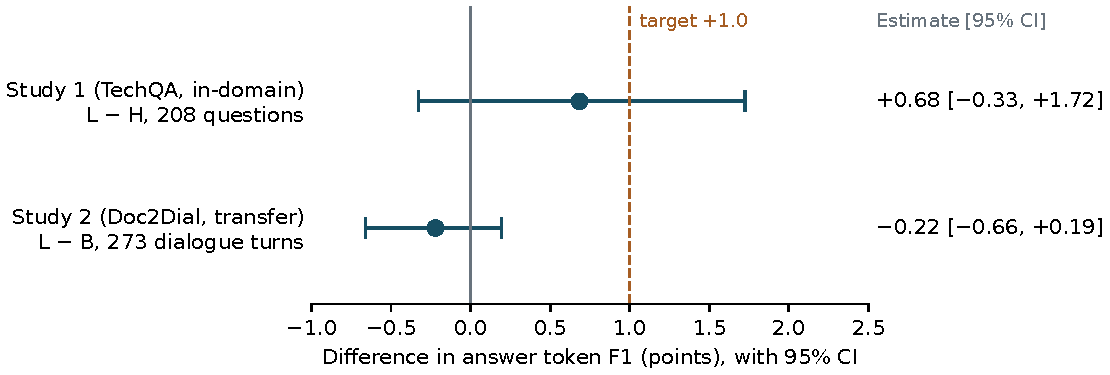
\includegraphics[width=\linewidth]{figures/primary_forest.pdf}
\caption{Primary estimates with 95\% intervals, in answer token-F1 points. Study~1 averages four chunkers per question with one generation seed (question bootstrap). Study~2 averages four chunkers and three paired training seeds per document (family bootstrap over 235 families). The dashed line marks the targeted $+1$-point gain.}\label{fig:primary}
\end{figure}
Neither study met its success criterion (Figure~\ref{fig:primary}). In Study~1, mean answer F1 was \SoneH\ for H and \SoneL\ for L, a difference of $\SoneDelta$ points computed from unrounded means (95\% CI $\SoneLow$ to $\SoneHigh$; $p=\SoneP$). Per-question differences were small and mixed: L was better on 115 questions, worse on 86 and tied on 7 (Cohen's $d_z=0.09$). Exact match was rare (1 of 832 H outputs and 4 of 832 L outputs). Because the interval runs from a small loss to gains above the target, Study~1 neither demonstrates nor excludes a one-point improvement. A post hoc breakdown by prior exposure gives $+0.16$ points for the 56 reserve questions without a discovered prior artifact and $+0.88$ for the 152 with one. These subsets are not randomized, so the difference does not establish a contamination effect (\supp{S4}{supp:study1}).

In Study~2, the $L-B$ difference in response F1 was $\StwoDelta$ points (95\% CI $\StwoLow$ to $\StwoHigh$; $p=\StwoP$). This is the more decisive negative result: conditional on the trained adapters, a gain of the targeted size lies outside the 95\% interval.

\subsection{Method means and variation in Study 2}
All three reranking methods have higher response F1 than hybrid retrieval, but adaptation adds little beyond the unadapted reranker (Table~\ref{tab:methods}): B exceeds U by only 0.02 points, and L is 0.20 points below U. Evidence NDCG@4 separates L from the other methods more clearly: L (\LNDCG) is below B (\BNDCG), U (\UNDCG) and H (\HNDCG).

The direction of the primary contrast is consistent across domains but not across training seeds. All four domain effects are negative (Table~\ref{tab:domains}), with an equal-domain mean of $-0.26$ points. The per-seed effects differ in sign (Table~\ref{tab:seeds}; standard deviation 0.49 points, range $-0.53$ to $+0.35$), although every leave-one-seed-out mean is negative. The positive effect at seed 20260904, which was also the grid-selection seed, reflects B's lowest seed mean (23.61 points, versus 24.42 and 24.11) rather than an unusually high L mean (23.58--23.96 across seeds; \supp{S3}{supp:study2}). The retrieval contrast does not change sign: L's evidence NDCG@4 is below B's for all three seeds. The answer contrast also varies by chunker, from $-0.99$ points (recursive-254) to $+0.41$ (\mbox{sentence-254}).
\begin{table}[htbp]\centering\small
\caption{Study 2 method means. F1 and exact match (EM) in points; NDCG@4 on the 0--1 scale. H/U: 1,092 records each; B/L: 3,276 each (three training seeds).}\label{tab:methods}
\begin{tabular}{lrrrr}\toprule
Method & Response F1 & Span F1 & Response EM & NDCG@4\\\midrule
H & 23.57 & 22.65 & 0.00 & 0.650\\
U & 24.03 & 23.30 & 0.18 & 0.686\\
B & 24.05 & 23.24 & 0.06 & 0.689\\
L & 23.83 & 23.12 & 0.06 & 0.612\\
\bottomrule\end{tabular}\end{table}

\begin{table}[htbp]\centering\small
\caption{Study 2 $L-B$ response-F1 difference by domain (points). The equal-domain mean weights domains equally; the primary estimand weights documents equally.}\label{tab:domains}
\begin{tabular}{lrr}\toprule
Domain & Documents & $L-B$ F1\\\midrule
DMV & 51 & $-$0.63\\
SSA & 77 & $-$0.11\\
Student aid & 50 & $-$0.18\\
VA & 95 & $-$0.11\\
Equal-domain mean & 273 & $-$0.26\\
\bottomrule\end{tabular}\end{table}


\subsection{From retrieval to answers}\label{sec:propagation}
In both studies, clear differences in NDCG@4 were not matched by clear differences in answer F1. The studies are not replications: they differ in comparator, population and protocol. In Study~1, L's NDCG@4 on the partly exposed reserve set exceeded that of hybrid retrieval for every training seed (0.807, 0.800 and 0.804 versus 0.769, with the corrected normalization; \supp{S4}{supp:study1}). Its answer-F1 gain for the one seed with generated answers ($\SoneDelta$ points) remains unresolved rather than absent (Figure~\ref{fig:primary}). In Study~2 the retrieval difference runs the other way: L's evidence NDCG@4 was 0.077 below B's, yet the response-F1 difference was small ($\StwoDelta$ points) and its interval included zero. For comparison, unadapted reranking (U) raised evidence NDCG@4 over H by 0.036 and response F1 by 0.46 points, less than half the targeted gain (\supp{S3}{supp:study2}).

The remaining analyses examine Study~2, where all four methods were compared. Exploratory analyses locate the retrieval differences in the ranking step rather than in the candidate pools. All methods rank the same pools, and these pools usually contain literal evidence: of 1,092 query--chunker pools, 874 contain at least one passage with a literal annotated grounding span, and 57 contain no graded passage at all. B and L also often choose the same passages: they share on average 67\% of their top four passages, and their top-four sets are identical in 20\% of paired cells. The fraction of cells whose packed context contains a literal annotated span is 0.704 for B and 0.670 for L (0.658 for H and 0.701 for U). Packing the selected passages into the generator's input loses no selected span: truncation was needed for only five of the 8,736 contexts, and two outputs reached the 512-token output cap (\supp{S5}{sec:s5}). Differences in what the generator receives therefore arise from which passages each method selects for its top four and in what order it ranks them.
\begin{table}[htbp]\centering\small
\caption{Study 2 $L-B$ response-F1 differences (points), leave-one-seed-out means, and retrieval NDCG@4 differences (0--1 scale). Seed 20260904 was also used for development-grid selection.}\label{tab:seeds}
\begin{tabular}{lrrr}\toprule
Seed & $L-B$ F1 & Without this seed & $L-B$ NDCG@4\\\midrule
20260904 & $+0.35$ & $-0.51$ & $-0.0827$\\
20260905 & $-0.48$ & $-0.09$ & $-0.0551$\\
20260906 & $-0.53$ & $-0.07$ & $-0.0937$\\
\bottomrule\end{tabular}\end{table}


A post hoc decomposition shows what L's evidence NDCG@4 deficit consists of (\supp{S5}{sec:s5}). L places fewer gold-document passages without a literal span in its top four than any other method (grade~1: 24.2\% of slots, versus 27.2--27.8\%) and more passages with no graded evidence (grade~0: 50.8\%, versus 46.0--48.1\%). Relative to H, L selects slightly more grade-2 passages (0.999 versus 0.986 per top four), yet its evidence NDCG@4 is 0.0379 lower, and grade-1 losses account arithmetically for 82.0\% of that gap. Relative to B, the gap comes from both grades in similar measure: 45.1\% from grade~1 and 54.9\% from grade~2. These decompositions are arithmetic and descriptive; they do not show that negative inversion caused the deficit.

Across the reported post hoc candidate-pool strata, answer differences do not consistently track retrieval differences. L's deficit relative to B is largest in the 161 pools that contain gold-document passages but no literal span ($-0.1427$ in NDCG@4), yet in those pools L's response F1 is 0.73 points higher than B's. In the 874 pools with a literal span, both differences are negative: $-0.0701$ in NDCG@4 and $-0.39$ F1 points.

In Study~2, differences in response F1 track response length more closely than retrieval quality. With each $L-B$ difference first averaged over a document's 12 chunker-by-seed cells, the response-F1 difference correlates weakly with the evidence-NDCG@4 difference (Pearson $r=0.22$; Spearman $\rho=0.18$) and more strongly, and negatively, with the difference in generated length ($r=-0.35$; $\rho=-0.47$; all associations in \supp{S5}{sec:s5}). These associations are descriptive and could also reflect question difficulty. Generated answers are much longer than the references. Under the F1 metric's normalized whitespace tokenization, reference utterances average 16.31 tokens (median 14), whereas generated answers average 63.80--65.60 tokens across methods; macro precision is 0.179--0.182 and recall 0.516--0.532. When a response overlaps the reference, adding nonoverlapping tokens lowers precision and F1 without lowering recall, so token F1 can penalize a longer answer that is no less supported.

\subsection{Compute and scoring cost}
Study~2 used 46,280 allocated A100-seconds (12.86 A100-hours, within the planned 20-hour budget), including loading, I/O, failures and retries. This total covers 12 grid jobs, 12 validation runs, six final refits, 1,092 retrieval cells, 152,880 reranker scores and 8,736 generated answers, but not development smoke tests or earlier project compute. Adapted reranking was slower than unadapted reranking in our offline measurements: the unadapted reranker scored 164.2 query--passage pairs per second in steady state, and the B and L adapters 91.6--91.7. These are timings of synchronized forward passes after tokenization, not per-request latencies or a matched serving comparison; per-seed measurements, generation throughput and the operational fixes made during the run are reported in \supp{S6}{supp:cost}.

\section{Discussion}\label{sec:discussion}
\subsection{What the studies establish}
On RQ1 and RQ2, neither study demonstrated, under its prespecified criterion, that the literal-match supervision pipeline improves answer F1. The two studies carry different weight, however. Study~1 compares L with hybrid retrieval on a partly exposed reserve set; its interval includes both zero and the targeted gain, so the in-domain answer effect remains unresolved. Study~2 asks the sharper question, literal-match against document-level supervision under transfer, and its interval excludes the targeted gain conditional on the trained adapters; it provides the more decisive negative result. Two features of the design make both results informative about that pipeline: the retrieval pipeline and generator were held fixed, with the same update budget for B and L in Study~2, and the protocols were frozen before comparative outcomes existed.

The success criterion was also demanding relative to what reranking achieved: the $+1$-point target was about twice the response-F1 gain of unadapted reranking over hybrid retrieval in Study~2. Under a retrospective normal-reference approximation, the gain detectable with 80\% power under the compound rule was 1.47 F1 points for Study~1 and 1.18 for Study~2, and a true one-point gain would have met the rule with a probability of only 47.7\% and 50.0\%, respectively. Because the rule required an observed gain of at least one point, under this approximation that probability could not exceed one half. These approximations condition on the observed variance; they are not exact power calculations for the sign-flip tests or prospective design claims (\supp{S1}{supp:register}).

The same design limits what the results can show. B and L are complete pipelines that differ in group composition and training exposure as well as in label values (Section~\ref{sec:labels}), so the comparison does not identify the effect of the labels alone. The nonsignificant answer difference between B and L is not evidence that the two pipelines are equivalent. Results from one retrieval setup, one generator and one answer metric also leave open whether literal-match labels would help in other settings and whether reranker adaptation helps in general.

For practitioners, the study gives no reason to prefer literal-match over document-level labels for adapting a reranker in this setting. Under transfer, it also gives no reason to adapt the reranker at all: U attains nearly the same response F1 as B, while adapted scoring was slower in our offline measurements and requires training. These measurements are not matched production benchmarks, and a deployment decision would still require task-specific validation and matched serving measurements.

\subsection{Possible explanations for the retrieval deficit}
The data are more definite about retrieval than about answers: under transfer, L had the lowest evidence NDCG@4 of the four methods and was below B for every training seed. A post hoc re-scoring suggests that L's deficit relative to B already appears in-domain, before transfer. We re-scored the saved TechQA validation rankings on L's own three-level grades; this uses one training seed and was not in the protocol. At the selected configuration, L scored 0.810 against B's 0.824 (difference $-0.013$ computed from unrounded values; 95\% question-bootstrap CI $-0.026$ to $-0.001$), and L was below B in five of the six grid configurations (\supp{S2.4}{sec:validationgrid}). The re-scoring is suggestive rather than confirmatory; if the in-domain deficit is real, an explanation of it should not rest on transfer alone.

Three features of the pipeline and its evaluation could produce such a deficit, and the study does not isolate any of them. The first is negative inversion: when a literal-match passage exists, L trains the reranker to rank gold-document passages without the literal answer below that passage, which may teach the reranker to demote useful passages. The transfer results fit this account descriptively, since L places the fewest grade-1 passages in its top four and its gap to H comes mostly from grade-1 losses (Section~\ref{sec:propagation}). How much inversion contributes is unclear, however, because fewer than a quarter of L's training groups contain a literal-match positive (Section~\ref{sec:labels}); the remaining groups pair grade-1 positives with grade-0 negatives, as in B.

The second is training exposure. With the same update budget, L covers a larger share of its smaller group inventory than B does (0.96 versus 0.43 of a pass; Section~\ref{sec:labels}), although at the selected budget neither method completes its first pass, and group construction changes how much weight each question receives. Model selection couples these exposure differences with the learning rate: L's own-grade optimum used the lower learning rate, for which no transfer result exists (Section~\ref{sec:training}).

The third is that transfer changes the evaluation target. Training uses technical-answer strings, Study~2 grades retrieval with grounding-span strings, and response F1 scores conversational agent utterances. The shift in domain and evaluation target may further contribute to the retrieval deficit observed under transfer, but it cannot explain the in-domain deficit that the post hoc re-scoring suggests. Separating these explanations would require new, development-only experiments that hold candidate pools, question weights and exposure fixed while comparing objectives such as multi-positive marginal likelihood \citep{zhang2025utility} or a graded ranking loss such as LambdaLoss \citep{wang2018lambda}. Such experiments would also need an evaluation population independent of the observed Doc2Dial outcomes.

\subsection{What the retrieval-to-answer gap means for evaluation}\label{sec:evaluation}
For RQ3, clear NDCG@4 differences corresponded to small or nonsignificant differences in answer F1 (Section~\ref{sec:propagation}). The document-level correlation between NDCG@4 and F1 differences is weak, consistent with what \citet{salemi2024} report for relevance-based retrieval evaluation and downstream RAG performance.

Two explanations fit this pattern, and the experiments cannot fully separate them. Under the first, \emph{weak propagation}, ranking differences change what the generator writes only slightly. Under the second, \emph{limited metric sensitivity}, the answers change more than token F1 can register, for example when a better-supported answer differs from the reference in wording or length. The Study~2 data bear on the second explanation, because token F1 depends on response length in this setting: generated answers are about four times as long as the reference utterances, and document-level F1 differences track length differences more closely than NDCG differences (Section~\ref{sec:propagation}).

The three comparisons in Section~\ref{sec:propagation} differ in whether retrieval metrics alone would have been a sufficient guide to the answer-level outcome. In Study~2, retrieval and answers both disfavored L relative to B: its evidence NDCG@4 was below B's for every training seed, in the same direction as its slightly lower response F1. In the other two comparisons, retrieval metrics would have been less informative: they favored L over hybrid retrieval in Study~1, where the answer effect remained unresolved, and favored unadapted reranking over hybrid retrieval in Study~2, where the response-F1 gain was a descriptive 0.46 points.

We therefore recommend that evaluations of reranker supervision measure the final answer, check first that the answer metric can register retrieval changes, and report retrieval and answer results side by side. Oracle-context and no-retrieval conditions are examples of such a check; neither condition is included in the present evaluation. This recommendation rests on one retrieval pipeline, one generator and one answer metric; it is not evidence that retrieval quality is unimportant for RAG. Testing it in other settings, including native multi-document dialogue tasks like MultiDoc2Dial \citep{feng2021multi}, would require a fresh evaluation split audited for prior exposure.

\section{Limitations}\label{sec:limitations}
\paragraph{Scope.} The studies use particular datasets, models, budgets and pipelines. They differ in preprocessing, model selection, comparator, number of seeds and exposure history, so their effects are not pooled or treated as replications. The shared configuration in Study~2 does not equalize which questions form groups or how often groups are seen.

\paragraph{Study 1 reserve exposure.} Earlier project work produced artifacts for 152 of the 208 reserve questions (16 with generated answers, 136 with retrieval only); 56 have no known prior artifact. The reserve also contains eight exact normalized duplicate questions, 31 near duplicates at token-set Jaccard $\ge 0.80$ (21 at $\ge 0.90$, 13 at $\ge 0.95$), and 44 questions whose gold documents (40 in total) also appear in development or validation. Artifact presence does not establish that a question was viewed, and its absence does not prove non-exposure. Pretraining exposure of the foundation models to TechQA or Doc2Dial is unknown.

\paragraph{Study 2 design.} Training uses single-turn TechQA answers, whereas transfer scores conversational agent utterances and grades retrieval with grounding spans. This changes both domain and target construct. The reranker instruction and generator prompt were written for single technical-support questions and were applied unchanged to serialized dialogue histories. One selected transition per document limits generalization across dialogue turns, and title-based families only approximate dependence between documents. Inference rests on 273 documents in 235 families, not on the 8,736 generated records. The interval resamples families with the three paired sets of trained adapters held fixed and so does not quantify uncertainty over future retraining seeds. Three seeds are insufficient for a precise estimate of that variation; the sign changes in Table~\ref{tab:seeds} remain material. The Doc2Dial evaluation set has now been observed and cannot serve as an untouched test.

\paragraph{Metrics.} Token F1 penalizes wording differences and can miss correct paraphrases, and agent utterances can include conversational material beyond the grounding span. In Study~2, generated answers are much longer than the reference utterances, so response F1 also depends on response length (Section~\ref{sec:propagation}); the weak association between retrieval and answer differences therefore cannot be attributed to weak propagation alone. Literal matching misses paraphrased or scattered evidence and can mishandle punctuation, numbers, commands and version strings. Gold-document membership is coarse, and a literal span in the context does not show that the generator used it. NDCG@4 reflects the grading convention described above, not an independent judgment of evidence quality. No human evaluation of answer quality is reported, so conclusions rest on automatic reference-based metrics.

\paragraph{Inference.} A non-significant result is not evidence of equivalence, and no equivalence test was planned. Secondary, exploratory and post hoc results (including the validation re-scoring in Section~\ref{sec:discussion}) are descriptive; the associations are not causal and could reflect confounding by question difficulty or output length.

\paragraph{Reproducibility.} Some training timers cover only a resumed session, and a legacy prompt-length field is invalid for 5,958 records (\supp{S5}{sec:s5}). No end-to-end deployment experiment or full-project compute total is available, and the public companion does not contain everything needed to rerun the experiments.

\section{Conclusion}
We tested whether adapting a reranker to prefer passages that literally contain the reference answer improves the answers of a fixed RAG generator. Neither study demonstrated such an improvement under its prespecified answer-F1 criterion. The more decisive evidence comes from transfer, where the literal-match reranker had slightly lower response F1 than a reranker adapted with document-level labels; conditional on the trained adapters, the 95\% interval for that difference excludes the targeted $+1$-point gain. The literal-match reranker also had the lowest evidence NDCG@4 of the four methods. In-domain, on a partly exposed reserve set, it improved NDCG@4 over hybrid retrieval, but its answer effect remained unresolved. Clear changes in retrieval ranking were not matched by clear changes in answer F1 in either study, and because token F1 also depended on response length, weak propagation and limited metric sensitivity cannot be fully separated.

These results concern the literal-match supervision pipeline as tested, with its training groups and training exposure, one retrieval setup, one generator and token F1 as the answer metric. They do not show that retrieval quality is irrelevant to answer quality or that reranker adaptation cannot help. For evaluating reranker supervision, the practical implication is to measure the final answer, to check first that the answer metric registers retrieval changes, and to report retrieval and answer results together.

\section*{Declarations}
\paragraph{Excluded rating exercise.} An earlier Study~1 human-rating exercise is excluded, and no human-rating results are reported or used.
\paragraph{Data and code availability.} Selected source code, aggregate results and the final pre-execution protocol for Study~2 are available at\\\url{https://github.com/zukhriddingit/chunkrag-reranking-study} (release v1.0.1);\\release v1.0.0 is archived at DOI \href{https://doi.org/10.5281/zenodo.22695835}{\mbox{10.5281/zenodo.22695835}}. The protocol was fixed before any comparative Doc2Dial outcome existed but was released afterward, so it is not a preregistration. The companion supports inspection of the selected source and aggregate results, not complete model-experiment replay: reflecting the chosen release scope, it omits exact split and selection records, per-record outputs, the six final adapters and some executed recovery code. The NVIDIA TechQA-RAG-Eval card lists Apache-2.0 and IBM's Doc2Dial distribution lists CC-BY-3.0; dataset text should be obtained upstream. Code and configurations are released under Apache-2.0 and aggregates, figures and documentation under CC-BY-4.0, as assigned per file (\supp{S7}{supp:repro}).
\paragraph{Funding and competing interests.} This study was self-funded. The authors declare no competing interests. This manuscript is a preprint and has not been accepted for journal publication.
\section*{Author contributions (CRediT)}
\noindent\textbf{Assylkhan Geniyat}: Conceptualization, Methodology, Software, Validation, Formal analysis, Investigation, Data curation, Visualization, Writing -- original draft, Writing -- review \& editing, Project administration.

\noindent\textbf{Zukhriddin Fakhriddinov}: Methodology, Validation, Formal analysis, Writing -- review \& editing.

\noindent\textbf{Atharv Gulati}: Validation, Writing -- review \& editing.

\section*{Declaration of generative AI and AI-assisted technologies in the manuscript preparation process}
During the preparation of this work the authors used OpenAI Codex (GPT-5.x and GPT-6.x series models) and Claude Code (Anthropic; Claude Opus 5.5) for drafting and language editing, manuscript organization and consistency checks. Two author-supplied Google Deep Review reports were used as review feedback; their suggestions were checked against the code and records. No generative image model was used. After using these tools, the authors reviewed and edited the content as needed and take full responsibility for the content of the publication.
